\documentclass[tikz,border=10pt]{standalone}
\usepackage{tikz}

\begin{document}
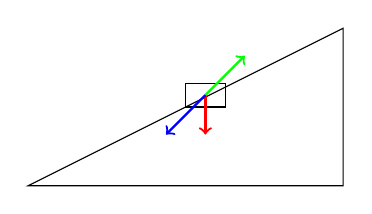
\begin{tikzpicture}

% Draw inclined plane
\draw (0,0) -- (4,2) -- (4,0) -- cycle;

% Draw rectangle (object) on the plane
\draw (2,1) rectangle ++(0.5,0.3);

% Draw forces
% Gravitational Force
\draw[->,red,thick] (2.25,1.15) -- (2.25,0.65);

% Normal Force
\draw[->,green,thick] (2.25,1.15) -- (2.75,1.65);

% Frictional Force
\draw[->,blue,thick] (2.25,1.15) -- (1.75,0.65);

\end{tikzpicture}
\end{document}